\documentclass{article}

\usepackage{graphicx}
\usepackage{tikz}
\usepackage{tikzsymbols}
\usetikzlibrary{calc,patterns,shapes.geometric}
\pagestyle{empty}
\usepackage[margin=0pt]{geometry}
\geometry{papersize={14in,12in}}

\def\centerarc[#1](#2)(#3:#4:#5){\draw[#1] ($(#2)+({#5*cos(#3)},{#5*sin(#3)})$) arc (#3:#4:#5);}

\begin{document}
	\begin{figure}
		\centering
		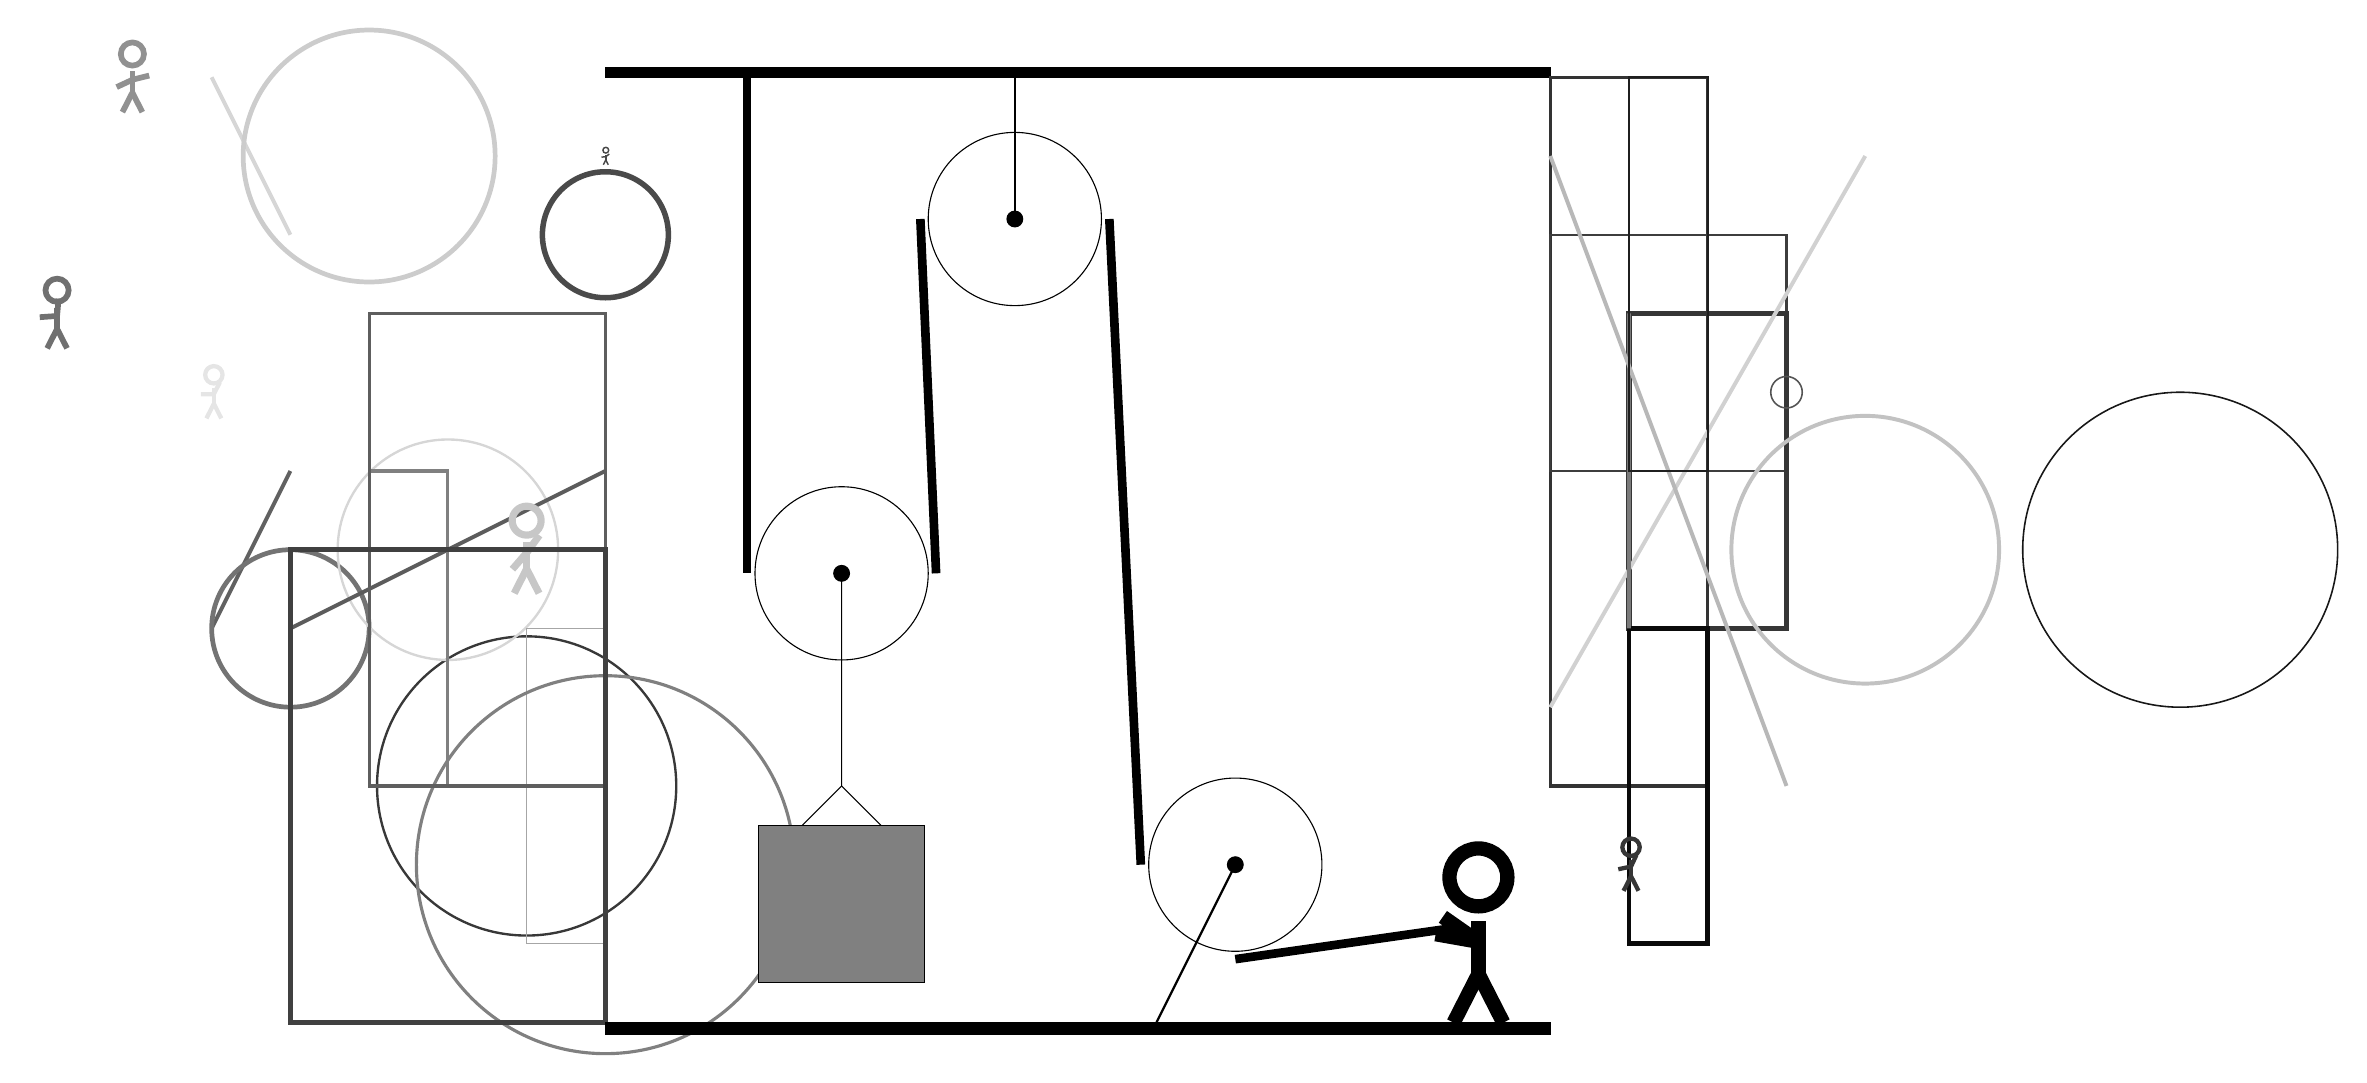
\begin{tikzpicture}
			%%%%% START %%%%%
			
			\draw[fill=black] (-2, 9) rectangle (10, 9.125);
			
			\draw[line width=0.3mm, color=black!66] (-2, -2) rectangle (-2, 4);
			
			\draw[line width=0.5mm, color=black!62](-7, 2) -- (-6, 4);
			\draw[line width=0.4mm, color=black!80] (10, 0) rectangle (12, 9);
			\draw[line width=0.5mm, color=black!16](-6, 7) -- (-7, 9);
			\draw [line width=0.3mm, color=black!78](-3, 0) circle (1.9);
			\draw[line width=0.3mm, color=black!76] (10, 7) rectangle (13, 4);
			
			\draw [line width=0.6mm, color=black!55](-6, 2) circle (1.0);
			
			\node[line width=0.5mm, color=black!72] at (-2, 8) {\Strichmaxerl[1][7][37]};
			\draw [line width=0.3mm, color=black!16](-4, 3) circle (1.4);
			\draw[line width=0.7mm, color=black!79] (11, 2) rectangle (13, 6);
			\draw[line width=0.2mm, color=black!35] (-2, -2) rectangle (-3, 2);
			\draw [line width=0.2mm, color=black!91](18, 3) circle (2.0);
			\draw[line width=0.5mm, color=black!64](-6, 2) -- (-2, 4);
			
			\draw [line width=0.2mm, color=black!67](13, 5) circle (0.2);
			\draw [line width=0.4mm, color=black!50](-2, -1) circle (2.4);
			\draw[line width=0.6mm, color=black!96] (12, -2) rectangle (11, 2);
			\node[line width=0.4mm, color=black!56] at (-9, 6) {\Strichmaxerl[4][4][85]};
			\draw [line width=0.6mm, color=black!20](-5, 8) circle (1.6);
			\node[line width=0.6mm, color=black!10] at (-7, 5) {\Strichmaxerl[3][1][63]};
			\draw[line width=0.5mm, color=black!18](14, 8) -- (10, 1);
			\node[line width=0.4mm, color=black!22] at (-3, 3) {\Strichmaxerl[5][49][54]};
			
			\node[line width=0.6mm, color=black!43] at (-8, 9) {\Strichmaxerl[4][25][14]};
			
			\draw [line width=0.5mm, color=black!24](14, 3) circle (1.7);
			\draw[line width=0.4mm, color=black!50] (-4, 0) rectangle (-5, 4);
			\draw[line width=0.4mm, color=black!63] (-2, 6) rectangle (-5, 0);
			
			\draw[line width=0.6mm, color=black!52] (11, 6) rectangle (11, 2);
			\draw[line width=0.5mm, color=black!28](10, 8) -- (13, 0);
			\draw [line width=0.7mm, color=black!71](-2, 7) circle (0.8);
			\draw[line width=0.2mm, color=black!88] (11, 9) rectangle (12, 4);
			\draw[line width=0.6mm, color=black!75] (-2, 3) rectangle (-6, -3);
			\node[line width=0.4mm, color=black!79] at (11, -1) {\Strichmaxerl[3][12][65]};
			
			
			\draw (3.2, 7.2) circle (1.1);
			\draw[fill=black] (3.2, 7.2) circle (0.1);
			\draw[thick] (3.2, 7.2) -- (3.2, 9);
			
			\draw (6, -1) circle (1.1);
			\draw[fill=black] (6, -1) circle (0.1);
			\draw[thick] (6, -1) -- (5, -3);
			
			\draw (1, 2.7) circle (1.1);
			\draw[fill=black] (1, 2.7) circle (0.1);
			
			\draw (1, 2.7) -- (1, 0) -- (0.5, -0.5);
			\draw (1, 0) -- (1.5, -0.5);
			\draw[fill=black!50] (-0.05, -0.5) rectangle (2.05, -2.5);
			
			\draw[line width=1.1mm] (-0.2, 9) -- (-0.2, 2.7);
			\centerarc[line width=1.1mm](1, 2.7)(180:360:1.2000000000000002);
			\draw[line width=1.1mm](2.2, 2.7) -- (2.0, 7.2);
			\centerarc[line width=1.1mm](3.2, 7.2)(0:180:1.2000000000000002);
			\draw[line width=1.1mm](4.4, 7.2) -- (4.8, -1);
			\centerarc[line width=1.1mm](6, -1)(180:270:1.2000000000000002);
			\draw[line width=1.1mm](6, -2.2) -- (8.8, -1.8);
			
			\node at (9, -1.9) {\Strichmaxerl[10][-35][170]};
			
			\draw[fill=black] (-2, -3) rectangle (10, -3.15);
			
			%%%%% END %%%%%
		\end{tikzpicture}
	\end{figure}	
\end{document}